\clearpage
\chapter{The LHCb detector}
\label{chap:dec}
The Large Hadron Collider (LHC) is a particle accelerator which accelerates protons along a $\sim$ 27km long tunnel which runs under the Franco-Swiss border. There are four detectors located at four different points on the \Gls{LHC}. These are \Gls{ATLAS}, \Gls{CMS}, \Gls{ALICE} and \Gls{LHCb}. At each one of these four points along the LHC, the protons beams are collided at a $pp$ collision or interaction point.


In this section, there will be a general overview of the LHCb detector, highlighting the aspects of the detector's design which allow for good $b$-physics performance. This is followed by a more detailed break down of the subdetectors relevant for this thesis, as well as an overview of the trigger system.




The \Gls{LHCb} detector is designed primarily to study $b$-physics. A profile of the detector is shown in~\autoref{fig:dec}. At the LHC, the majority of $b\overline{b}$ quark pairs are produced at low values of $\theta$, where $\theta$ is defined as being equal to $0$ along the $z$ axis in~\autoref{fig:dec}. The LHCb detector is a single-arm spectrometer in the sense that there is no instrumentation about $\theta = \pi$.



%% The LHCb experiment is the world's first $b$-physics experiment at a hadron collider.

 %% where $\theta$ is defined as being equal to $0$ along the $z$ axis in~\autoref{fig:dec} and sweeping through the $z$-$y$ plane.
\begin{figure}[!h]
  \centering
  \includegraphics[scale = 0.6]{figs/lhcdetector}
  \caption{A profile of the LHCb detector \cite{det_paper}. Any reference to $x, y ,z$ directions in this thesis refers to this diagram. The interaction point is located inside the Vertex Locator. %is at $z \sim$ 0\mm.
  }
  \label{fig:dec}    
\end{figure}


By placing the detector instrumentation along the beamline, the LHCb detector exploits the fact that the $b\overline{b}$ quark pairs are produced at low values of $\theta$, or high values of pseudorapidity, $\eta$, where

\begin{equation}
  \eta = -\ln[\tan\frac{\theta}{2}].
\end{equation}
%The relationship between $\theta$ and $\eta$ can be seen in~\autoref{fig:eta}.
%% \begin{figure}[!h]
%%   \centering
%%   \includegraphics[scale = 0.4]{figs/eta.png}
%%   \caption{Polar angle $\theta$ vs pseudorapidity \cite{wikieta}.}
%%   \label{fig:eta}    
%% \end{figure}
The production of $b\overline{b}$ pairs as a function of $\eta$ can be seen in~\autoref{fig:bbtheta}.
\begin{figure}[!h]
  \centering
  \includegraphics[scale = 0.4]{figs/bb_theta_2D}
  \caption{The production of $b\overline{b}$ quarks as a function of $\eta$. The acceptance for LHCb and General Purpose (\Gls{GP}) detectors are overlaid on top. Figure taken from the LHCb public page.}
\label{fig:bbtheta}    
\end{figure}
The LHCb coverage in $\eta$ ($2<\eta<5$) is also shown in~\autoref{fig:bbtheta}, along with a comparison of the $\eta$ coverage of the general purpose (GP) detectors, ATLAS and CMS. % as demonstrated in~\autoref{fig:bbtheta}. % and~\autoref{fig:cmslhcb}.
%% \begin{figure}[!h]
%%   \centering
%%   \includegraphics[scale = 0.4]{figs/CMS_LHCb.jpg}
%%   \caption{Comparing the layout of the CMS and LHCb detectors with respect to the $pp$ interaction point \cite{bbtheta}.}
%% \label{fig:cmslhcb}
%% \end{figure}
Despite LHCb only covering 1.8\% of the total solid angle, 27\% of $b\overline{b}$ pairs fall within the detector acceptance \cite{LHCb-DP-2014-001}. 

%% Another contrast between LHCb and other LHC experiments is the detector's design luminosity.
%% The instantaneous luminosity is defined as
%% \begin{equation}
%%   \rm{L}_{int}  = \frac{1}{\sigma} \frac{dN}{dt},
%% \end{equation}
%% where $\sigma$ is the $pp$ interaction cross section  which is a function of the centre of mass energy, as shown in~\autoref{fig:ppxs}.
%% \begin{figure}
%%   \centering
%%   \includegraphics[scale = 0.4]{figs/pp_xsection.png} 
%%   \caption{The $pp$ cross-section, $\sigma_{pp}$ as a function of centre of mass energy, where $s$ is the Mandelson variable defined as $s = (p^{1}_{\mu} + p^{2}_{\mu})^{2}$ \cite{pdg_hxs}.}
%%   \label{fig:ppxs}
%% \end{figure}
A key method for distinguishing $b$-hadrons from other particles is to measure the displacement of particles in the detector, as $b$-hadrons tend to be highly boosted. A high number of tracks at any time makes obtaining a good resolution on the displacement of these vertices difficult. As a consequence, the luminosity collected by the LHCb detector is lower than other LHC experiments.  At the LHCb experiment an integrated luminosity of 1 \invfb of data was collected during 2011, with $\sqrt{s}$ = 7~\tev.  During 2012, 2 \invfb of data was collected, with $\sqrt{s} = $ 8~\tev. The data collected during the years 2011 and 2012 at the LHC is referred to as Run-1 data.  Data collected during the years 2015 and 2016 is referred to as Run-2 data.%As a comparison, the integrated luminosity for ATLAS was $\sim$ 20 \invfb for the year of 2012 alone \cite{atlasfb}.%\url{https://twiki.cern.ch/twiki/bin/view/AtlasPublic/LuminosityPublicResults#Integrated_luminosity_summary_pl}.
%The data collected during the years 2011 and 2012 at the LHC is referred to as Run-1 data. At LHCb, for Run-1 data, the average luminosity is given by \cite{int_L}
%% \begin{equation}
%%    \rm{L}_{int} = (2 \ldots 4) \cdot 10^{32}/cm^{2}/s = (0.2 \ldots 0.4)\,nb^{-1}/s.
%% \end{equation}

%There is an integrated luminosity ($\rm{L} \equiv \int\!\mathcal{L}_{int}\,\mathrm{dt}$)

%% The LHCb detector has a lower design luminosity in order to reduce occupancy (the number of particles traversing a detector cell per event) and pile-up (a function of the number of visible $pp$ interactions per bunch crossing) as well as reducing radiation damage.  This reduced occupancy and pile-up makes it easier to gain more precise knowledge about each individual event. 
   
The detector subsystems, all marked in~\autoref{fig:dec}, can be outlined as follows:
\begin{description}
\item [VELO] The Vertex Locator system (\Gls{VELO}) is a high precision tracking system which provides good resolution on the $pp$ interaction vertex, or primary vertex (\Gls{PV}), and flight distance (\Gls{FD}). The resolution of the flight distance (i.e. how far a particle flies before decaying) for particles produced at the PV (so-called \gls{prompt} decays) is a function of the PV and the Secondary Vertex (SV). The VELO is discussed in more detail in~\autoref{sec:velo}.
\item [TT and T stations] The tracking system is completed by the Tracker Turicensis (TT) station and Tracking stations (T stations), which lie upstream and downstream of the magnet respectively. The tracking system is discussed in more detail in~\autoref{sec:Tst} %and is made up of silicon microstrips and the tracking stations (T stations), which lie after the magent and are made up of silicon mircostrips in the inner parts and Kapton/AI straws in the outparts. 
\item [RICH 1,2] The two Ring Imaging Cherenkov detectors (\Gls{RICH}) provide identification of charged hadrons by using Cherenkov radiation. The RICH information is important in the \Lbpi analysis, to help distinguish pions and protons from kaons. The RICH is discussed in more detail in~\autoref{sec:rich}.
\item [The ECAL, HCAL and SPD/PS] The calorimeter system provides identification of photons, electrons (\Gls{ECAL}) and hadrons (\Gls{HCAL}) as well as giving information on their position and energy. The pre-shower (\Gls{PS}) detectors and Scintillator Pad Detectors (\Gls{SPD}) are used to help electron identification. The information provided by the calorimetry system is less important to the \Lbpi analysis than other subdetectors and is not discussed further.
\item [Muon Chambers]  The muon chambers identify muons by employing large amounts of iron, which stop most particles, but not muons. The process of muon identification is discussed in more detail in~\autoref{sec:muonID}.
\end{description}

In addition to these subdetectors there is also the magnet, as marked in~\autoref{fig:dec}, which provides a strong magnetic field, bending charged particles in the $x - z$ plane. % in~\autoref{fig:dec}, allowing the momentum of particles to be measured.

%% As the analyses in this thesis use Run-1 data only, the description of the detector in this chapter refers to the specific set-up and configuration of the trigger and detector as used during Run-1.
Before discussing the detectors subsystems in detail the key features of the trigger are outlined. The purpose of the trigger is to reduce the amount of data read out from the detector to a manageable level, whilst still preserving the most interesting physics events.
\section{Trigger}
\label{sec:trig}
The LHCb trigger consists of two levels, the hardware trigger, referred to as the Level-0 (\Gls{L0}) trigger and the software trigger referred to as the High Level Trigger (\Gls{HLT}). The L0 trigger makes decisions based on information from the muon systems and the calorimeter and reduces the rate of events to below 1\mhz, at which point the whole detector can be read out. The HLT reduces the rate down to 5 \khz, at which point events can be stored. %Stored events are later reconstructed more accurately and a further selection is applied. This processing of stored events is referred to as off-line reconstruction and off-line selection.
An overview of the HLT algorithms and the rates involved in the entire trigger process in 2012 can be seen in~\autoref{fig:trig_alg}.

 %The HLT trigger is split into two stages, referred to as HLT1 and HLT2
%% \begin{figure}[!h]
%%   \centering
%%     \includegraphics[]{figs/L0.png} 
%%   \caption{Overview of the Level-0 trigger. The numbers indicate the number of channels between the input and processing system (Trigger or Pile-up system) \cite{det_paper}. %Every 25 ns the pile-up system receives 2048 chan-nels from the pile-up detector, the Level-0 calorimeters 19420 channels from the scintillating paddetector, preshower, electromagnetic and hadronic calorimeters while the Level-0 muon handles25920 logical channels from the muon detector. \cite{det_paper}The 
%%   }
%%   \label{fig:L0}
%% \end{figure}

\begin{figure}[!h]
  \centering
    \includegraphics[scale = 0.5]{figs/LHCb_Trigger_RunIAlgDetail} 
  \caption{Overview of the LHCb trigger rates. Figure taken from the LHCb public page.}% of the Level-0 trigger. The numbers indicate the number of channels between the input and processing system (Trigger or Pile-up system) \cite{det_paper} %Every 25 ns the pile-up system receives 2048 chan-nels from the pile-up detector, the Level-0 calorimeters 19420 channels from the scintillating paddetector, preshower, electromagnetic and hadronic calorimeters while the Level-0 muon handles25920 logical channels from the muon detector. \cite{det_paper}
  
  \label{fig:trig_alg}
\end{figure}



\subsection{L0 trigger}
\label{sec:L0trig}
The L0 trigger is divided into the L0-Calorimeter trigger, the L0-Muon trigger and L0-PileUp trigger, the latter being used only for the determination of the luminosity. The L0 trigger is fully synchronised with the 40\mhz bunch crossing rate of the LHC.

%% The L0-Calorimeter trigger builds three types of candidates by using various combinations of hit clusters within the SPD, PS, ECAL and HCAL. These candidates are \texttt{L0Hadron}, \texttt{L0Photon} and \texttt{L0Electron}. If an event contains at least one candidate whose transverse energy, $E_{T}$, meets the requirements in~\autoref{tab:L0}, the event is retained. 

%% \begin{table}
%%   \centering

%%     \begin{tabular}{|l|c|c|}
%%       \hline
%%       Variable &$P_{T}$ or $E_{T}$&$P_{T}$ or $E_{T}$\\
%%       Year &2011&2012\\
%%       \hline
%%       single muon & 1.48\gevc&1.76\gevc\\
%%       dimuon $P_{T_{1}}$ $\times$ $P_{T_{2}}$ & $(1.30\gevc)^{2}$& $(1.60\gevc)^{2}$\\
%%       hadron & 3.50\gevc& 3.70\gevc\\
%%       electron & 2.50\gevc& 3.00\gevc\\
%%       photon & 2.50\gevc& 3.00\gevc\\
%%       \hline
%%     \end{tabular}
%%       \caption{Typical L0 thresholds used in Run-1 for different candidate types.}
%%     \label{tab:L0}
%% \end{table}
The events that pass the LHCb trigger can be split into three categories. Triggered On Signal (\Gls{TOS}) events are those for which the presence of the signal candidate is sufficient to fire the trigger. Triggered Independent of Signal (\Gls{TIS}) are those events whereby the trigger is fired without using any of the hits associated with the signal particles. Finally, there are events that are neither TIS nor TOS, i.e. neither the presence of the signal alone nor the rest of the event alone are sufficient to fire the trigger, but rather both are necessary \cite{LHCb-PUB-2014-039}. These are referred to as \Gls{TISTOS} events.

%% The muon L0 trigger looks in each quadrant of the muons stations and if the $P_{T}$ of a single muon, or the combination of the first and second highest $P_{T}$ muon in a single quadrant, meets the requirements in~\autoref{tab:L0}, the event is retained.
%% Trigger events can be classed into two cateogories

In the \Lbpi analysis a TOS is required on the L0 line \texttt{L0Muon}, which requires the $P_{T}$  of single muon in an event to be above 1.48\gevc in 2011 data \cite{2011trig} and 1.76 \gevc in 2012 data.

The TOS efficiency of the 2011 \texttt{L0Muon} line, calculated using \Bu\to\jpsi(\mup\mun)$\kaon^{+}$ data via the so-called TISTOS technique, outlined in~\autoref{sec:tistos}, is shown in~\autoref{fig:L0eff}, as a function of the $P_{T}$ of the \jpsi.
\begin{figure}
  \centering
  \includegraphics[scale = 0.4]{figs/L0trig2012data.pdf}%L0Muoneff.png}
  \caption{The 2011 \texttt{L0Muon} and \texttt{L0DiMuon} lines efficiency, $\epsilon_{TOS}$, on \Bu\to\jpsi(\mup\mun)$\kaon^{+}$ as a function of $P_{T}$ (\jpsi)\cite{LHCbperf}.
  }
  \label{fig:L0eff}
\end{figure}




\section{The HLT trigger}
\label{sec:hlttrig}
The HLT trigger consists of two levels, Level-1 and Level-2, referred to as HLT1 and HLT2 respectively. The HLT1 performs a partial event reconstruction and an inclusive selection of signal candidates, reducing the rate to 80\khz. The HLT2 performs a full event reconstruction which is close to that used for the off-line reconstruction and reduces the rate to 5\khz.

The HLT1 trigger decisions most relevant to the \Lbpi analysis are the \texttt{Hlt1TrackAllL0} and \texttt{Hlt1TrackMuon} lines. The \texttt{Hlt1TrackAllL0} line selects VELO track candidates based on their $P_{T}$ and displacement from the primary vertex. If the selected VELO track also matches with hits in the muon chamber and has a $P_{T}>1\gevc$ then it will be selected by the \texttt{Hlt1TrackMuon} line \cite{trigperf}. The efficiency of the \texttt{Hlt1TrackAllL0} and \texttt{Hlt1TrackMuon} trigger lines can be seen in~\autoref{fig:HLT1eff}.%%%%% ($P_{T}>1.6\gevc$)

\begin{figure}
  \centering
    \subfloat[]{\includegraphics[scale = 0.27]{figs/2012dataHLTtrackALLL0.png}\label{1}}%L0Muoneff.png}
    \subfloat[]{\includegraphics[scale = 0.27]{figs/2012dataHLTtrackmuon.png}\label{2}}%L0Muoneff.png}
    \caption{The \texttt{Hlt1TrackAllL0} TOS efficiency ($\epsilon_{TOS}$) of the decays indicated in the legend as a function of the $P_{T}$ of the relevant $\B$ or $D$ meson, \protect\subref{1}, the \texttt{Hlt1TrackMuon} (and \texttt{Hlt1DiMuonHighMass}, \texttt{Hlt1DiMuonLowMass}) $\epsilon_{TOS}$ as a function of the $P_{T}$ of the \jpsi \protect\subref{2}. Both plots show 2012 data \cite{trigperf}.
  }  \label{fig:HLT1eff}
\end{figure}

%% then this track will be selected by the \texttt{Hlt1TrackMuon} line, providing that it is a good quality candidate with $P_{T}>1\gevc$.  Candidates are required to pass at least one of either the \texttt{Hlt1TrackAllL0} or \texttt{Hlt1TrackMuon} line in the \Lbpi analysis.
   
The HLT2 trigger consists of so-called topological lines, named \texttt{Hlt2Topo(N)Body}, which are designed to trigger on partially reconstructed $b$-hadron decays. The selection of partially reconstructed decays allows heavy flavour decays to be selected even in the cases where not all the final state particles are reconstructed.    
To allow for an inclusive cut on partially reconstructed events, a corrected mass \gls{mcorr} is used that takes into account the amount of missing transverse-momentum with respect to the flight of the mother ($P_{T^{\prime} miss}$). This is defined as
\begin{equation}
  m_{corr} = \sqrt{m^{2} + {P_{T^{\prime} miss}}^{2}} + P_{T^{\prime}miss}.
\end{equation}

The topological lines use a Boosted Decision Tree (\Gls{BDT}) \cite{miniboone} to discriminate between signal and background. A BDT employs multivariate analysis techniques to combine a set of discriminating variables into a single discriminating variable. A more detailed overview of BDTs is given in Appendix~\ref{app:bdt}. Due to the detector resolution and the need to account for any variation in, for example, the detector efficiency, a BDT which receives input variables that have been discretised is preferred. These BDTs which take discrete input variables are referred to as a Bonsai BDT (\Gls{BBDT})\cite{bonsai}. The BBDT lines used in the \Lbpi analysis are \texttt{Hlt2Topo2BodyBBDT} and \texttt{Hlt2TopoMu2(3)BodyBBDT}, which select two or three body candidates respectively. The variables used in the BBDT are $\sum|P_{T}|$, $P^{min}_{T}$, $mass$, $m_{corr}$, \Gls{DOCA}, \gls{ipchi2} and \gls{fdchi2}\cite{BBDTstuff}\cite{Puig:1970930}. The $FD\chisq$ is defined for two vertices (generally the PV and SV) as the change in $\chisq$ when the two vertices are combined into a single vertex fit. The DOCA is the distance of closest approach between two tracks. The impact parameter (\Gls{IP}) is defined as the distance between a track and the PV at the track's closest point of approach, as sketched in~\autoref{fig:IPFD}. The $IP\chisq$ is the difference in the $\chisq$ of the vertex fit to the PV, when the track whose $IP\chisq$ is being measured is added and removed from the fit.

\begin{figure}[!h]
  \centering
  \includegraphics[scale = 0.4]{figs/PVFD_def.png} 
  \caption{The Flight Distance (FD), Impact Parameter (\Gls{IP}) and Primary and Secondary Vertices (PV, SV) for an event. The black lines labelled $p$ represent the colliding proton beams. Image altered from Ref.~\cite{Sam}.}
  \label{fig:IPFD}
\end{figure}





%% along with the cuts placed on them, are shown in~\autoref{tab:BBDT}.

%% In~\autoref{tab:BBDT}, the $\mathrm{FD}_{\chisq}$ is defined for two vertices (generally the PV and SV) as the change in $\chisq$ when the two vertices are combined into a single vertex fit. The DOCA is the distance of closest approach between two vertexed tracks and the $IP_{\chisq}$ is the difference in the $\chisq$ of the fit to the PV, when the track whose $IP_{\chisq}$ is being measured is added and then removed.



 
%% \begin{table}
%%   \centering
%%   \begin{tabular}{|c|c|}
%%     \hline
%%     Variable & Cuts (2,3,4-body)\\
%%     \hline
%%     $\sum|P_{T}|$[\gevc]& $>$2,4,4\\
%%     $P^{min}_{T}$[\gevc]& $>$0.5 \\
%%         $m$ [\gevc] &$<$7 \\
%%     $m_{corr}$[\gevcc] &\\
%%     $DOCA[\mm]$ & $<$0.2\\
%%     $IP_{\chisq}$ & \\
%%     $FD_{\chisq}/100$ & $>$1 \\
%%     \hline
%%   \end{tabular}
%%   \label{tab:BBDT}
%% \end{table}

 %% which allows for a reduced CPU time and a more stabilty. The discreteized BDT's are referred to as Bonzai Boosted Decision Tree's (BBDT) 

Similar to the HLT1 algorithm, the HLT2 algorithm has lines that select events with one or two identified muons in the final state. The criteria of the HLT2 muon lines relevant for the \Lbpi analysis are shown in~\autoref{tab:hlt2Mu}. The criteria in~\autoref{tab:hlt2Mu} are split into \texttt{Detached} and \texttt{DetachedHeavy} lines, with the latter having a higher threshold on the dimuon mass.
\begin{table}

  \centering
  \begin{tabular}{|l|c|c|}
    \hline
    \texttt{Hlt2DiMuon}& \texttt{Detached} & \texttt{DetachedHeavy}\\
    \hline
    Track $\chisq/\mathrm{ndof}$ & $<5$  & $<5$\\
    Track $IP_{\chisq}$ & $>9$ & - \\
    Mass [\gevcc] & $>1$ & $>2.95$ \\
    $FD_{\chisq}$ & $>49$ & $>25$ \\
    $\mathrm{vertex}_{\chisq}$ & $<25$ & $<25$ \\
    $P^{\mu\mu}_{T}$[\gevc] & $>1.5$ & - \\
    \hline
  \end{tabular}
    \caption{The HLT2 lines used in the \Lbpi analysis based on two identified muons \cite{2011trig}.}
  \label{tab:hlt2Mu}
\end{table}


%%  along with the efficiency of several  of the HLT2 topological lines.

%% \begin{figure}[!h]
%%   \centering
%%   \includegraphics[]{figs/topomu.png}   
%%   \caption{}
%%   \label{fig:AllL0zcite{2011trig}}
%% \end{figure}

\subsection{The TISTOS method for efficiency estimations}
\label{sec:tistos}
There are two ways of estimating the trigger efficiency, using simulation to reproduce fully the physics and detector, or using a data driven approach. In the data driven case, as the detector records only events passing the trigger, the number of events that the trigger processes is not directly observable. A solution to this is to look at and compare samples which fire the trigger in different ways. As previously discussed, the accepted trigger events can be split into three categories: TIS, TOS and TISTOS. %% Triggered On Signal (TOS) events are those for which the presence of the signal is sufficient to fire the trigger. Triggered Independent of Signal (TIS) are those events whereby the trigger is fired without using any of the hits associated with the signal particles. Finally, there are events that are neither TIS nor TOS, that is, neither the presence of the signal alone nor the rest of the event alone are sufficient to fire the trigger, but rather both are necessary \cite{LHCb-PUB-2014-039}. There are referred to as TISTOS events.

The TIS and TOS events can be used to predict the efficiency of the TOS sample, $\epsilon_{TOS}$, if it is assumed that the TIS and TOS events are independent. Under this assumption then the trigger efficiency under TOS given that the event is TIS, $\epsilon_{TOS|TIS}$, is simply $\epsilon_{TOS|TIS} = \epsilon_{TOS} $ giving

\begin{equation}
  \epsilon_{TOS} = \frac{N_{TISTOS}}{N_{TIS}}.
\end{equation}
%% The efficiencies referred to in the following trigger sections have been calculated using this so-called TISTOS data-driven method.
Thus the efficiency for TOS events can be deduced by looking at the number of TOS events which are triggered under TIS.


\FloatBarrier

\section{The VELO}
\label{sec:velo}
This section is based on sections 5.3 and 5.4 of Ref.~\cite{LHCb-DP-2014-001}.

The VELO provides $R$ and $\phi$ coordinates by using silicon modules placed along the beam direction, as shown in the upper half of~\autoref{fig:VELO}. The modules act as sensors in the $R$ and $\phi$ directions. Once beam conditions are stable, the VELO sensor is placed 7\mm from the collision point. This is narrower than the aperture required for injection by the LHC. Thus during injection the VELO is opened, again as indicated in~\autoref{fig:VELO}. The VELO is designed such that tracks within the nominal LHCb acceptance cross at least three VELO stations.
\begin{figure}[!h]
  \centering
    \includegraphics[scale = 0.3]{figs/VELO.png} 
  \caption{Above: the VELO stations as placed along the $z$ direction, below: as shown in the $x-y$ plane in both the open (for injection) and closed (for stable beams) configuration\cite{det_paper}. %Every 25 ns the pile-up system receives 2048 chan-nels from the pile-up detector, the Level-0 calorimeters 19420 channels from the scintillating paddetector, preshower, electromagnetic and hadronic calorimeters while the Level-0 muon handles25920 logical channels from the muon detector. \cite{det_paper}
  }
  \label{fig:VELO}
\end{figure}

\subsection{Measuring the impact parameter}
The impact parameter is an important variable in the \Lbpi analysis, as it allows \gls{prompt} background to be distinguished from signal candidates. The resolution depends on, amongst other things, the amount of multiple scattering of particles by the detector material and the resolution of the position hits in the detector from which the tracks are reconstructed. The resolution as a function of $1/\pt$ can be seen in~\autoref{fig:IP}. Tracks with $\pt>1\gevc$ have a resolution of $<35\mum$.


\begin{figure}
  \centering
  \subfloat[]{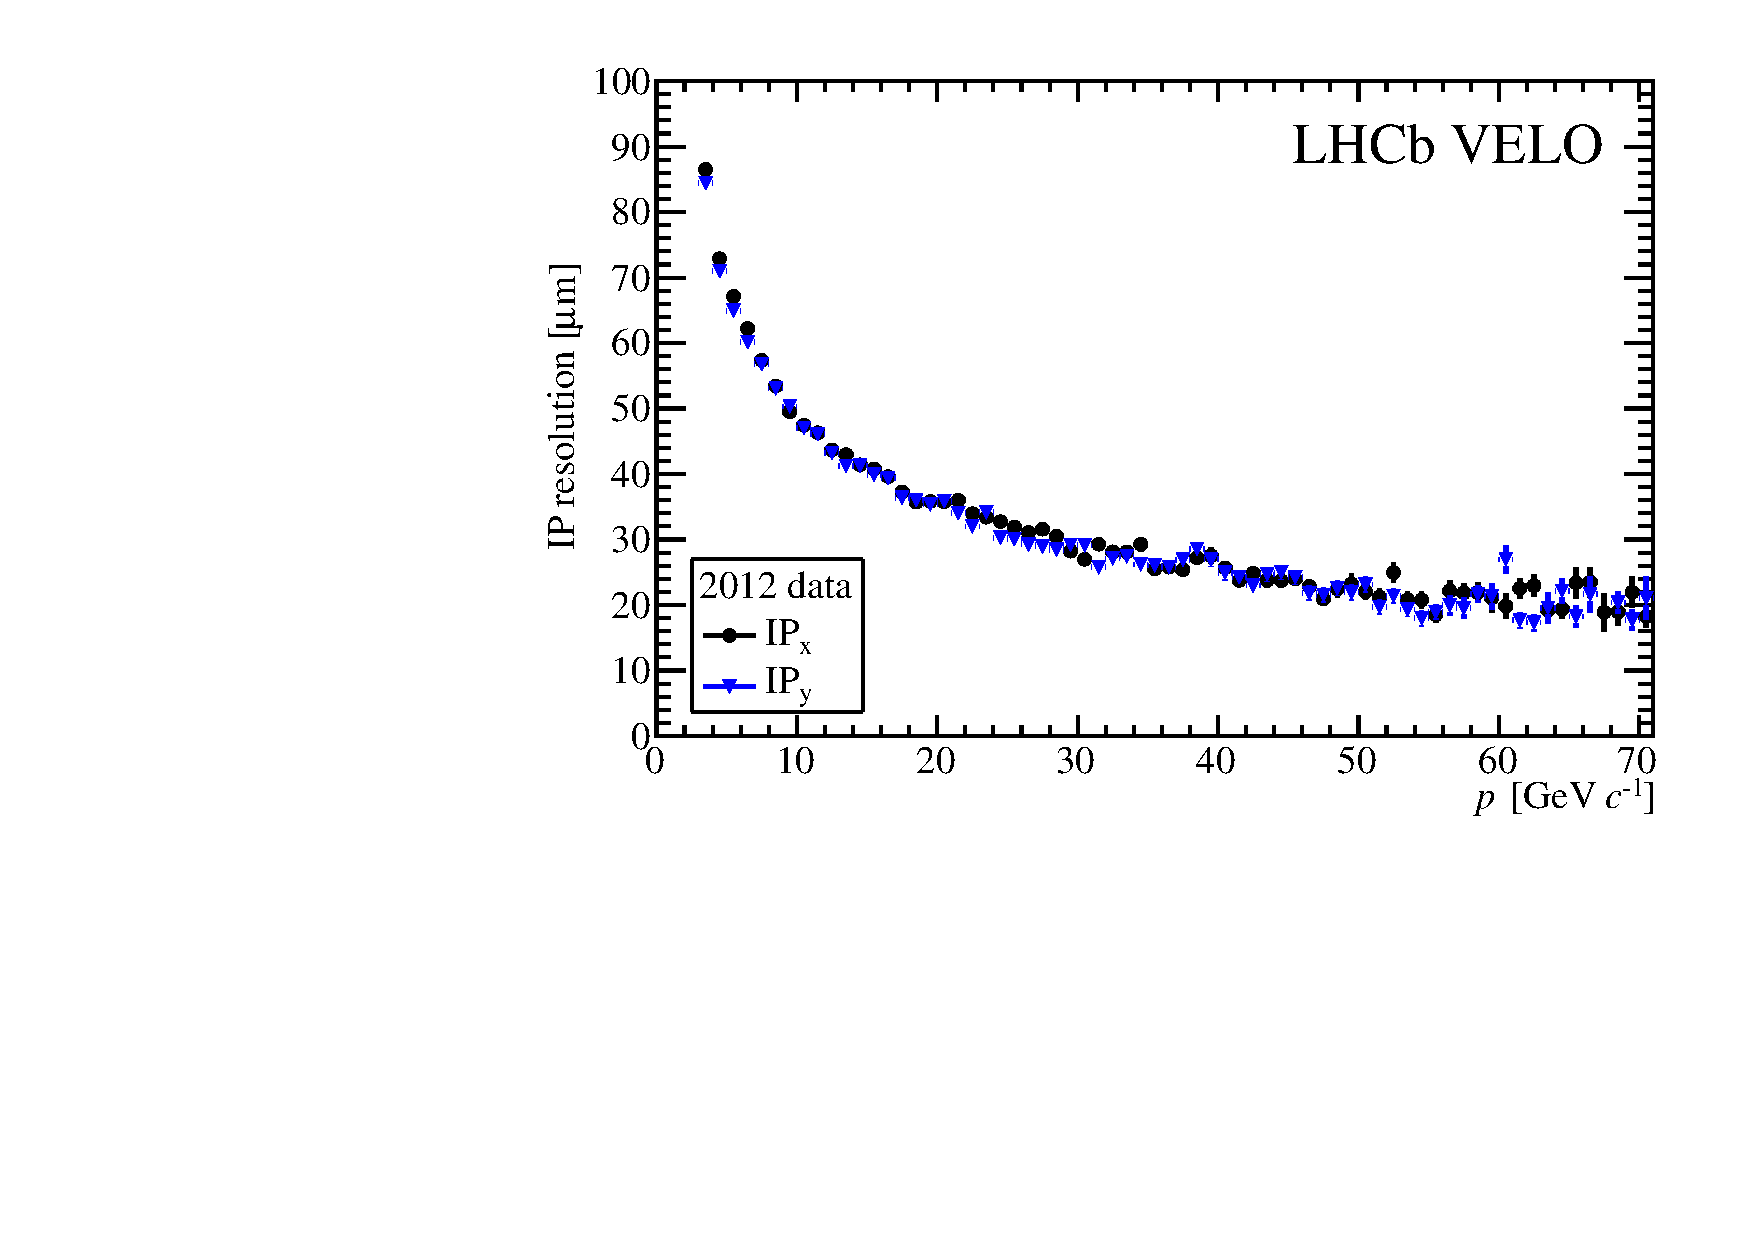
\includegraphics[scale = 0.4]{figs/IPRes-Vs-P-CompareIPxIPy-2012}\label{1}}
  \subfloat[]{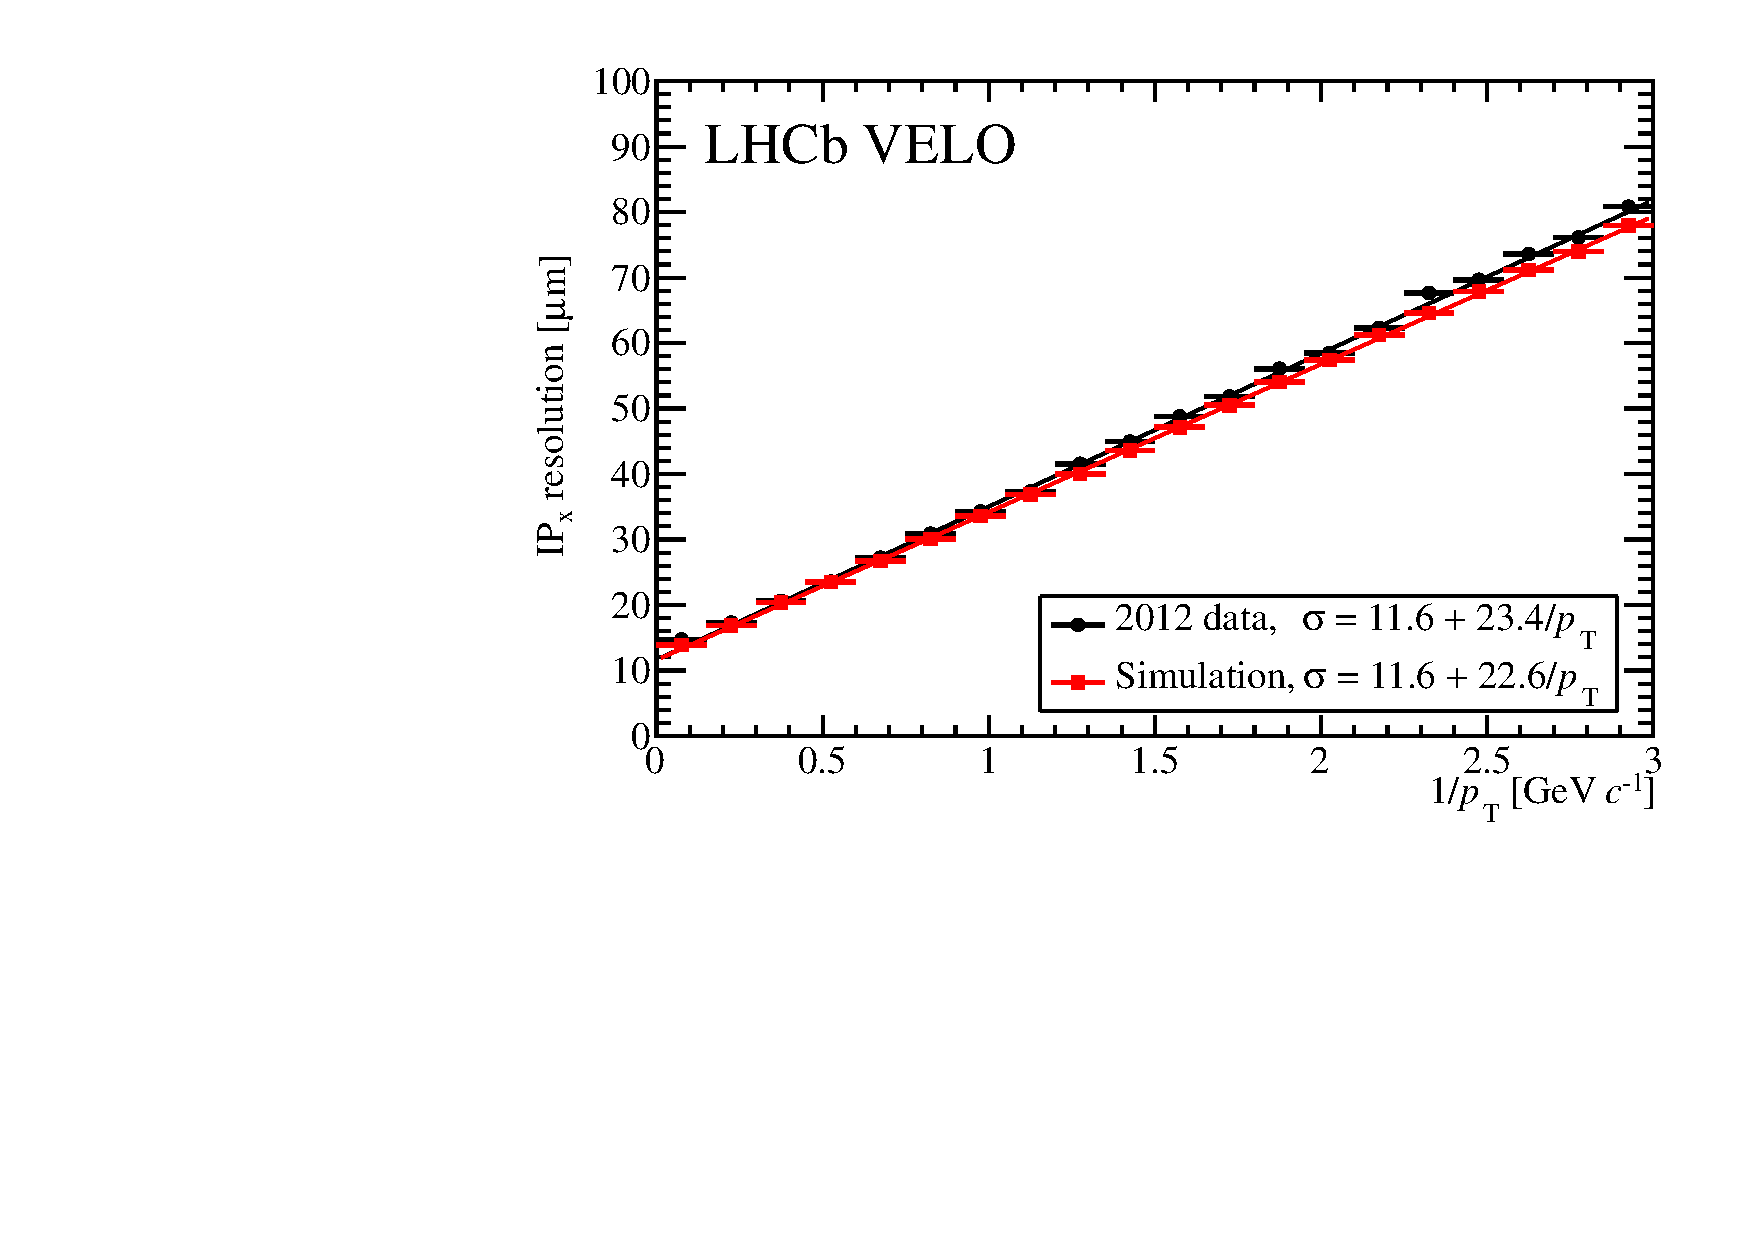
\includegraphics[scale = 0.4]{figs/IPXRes-Vs-InversePT-Compare2012DataToMC}\label{2}}
  \caption{The resolution of $IP_{x}$ and $IP_{y}$ as a function of the momentum of the track, \protect\subref{1}, the resolution of $IP_{x}$ and $IP_{y}$ as a function of $1/P_{T}$, \protect\subref{2} \cite{LHCb-DP-2014-001}.}
  \label{fig:IP}
\end{figure}

\subsection{Measuring the PV position}
A good measurement of the PV position is important for gaining good precision on the FD of a particle. The PV resolution is strongly correlated with the number of tracks, $N$, in an event. At least five tracks are required to form a PV. %The maximum number is around 100.

The resolution of the PV in the $x$, $y$ and $z$ directions is fitted using the function
%% is deduced by randomly splitting the tracks in an event into two sets. The vertex reconstruction algorithm is then applied to each set and vertices in each set which are have a difference in their $z$ position of less than $2\mm$ are deemed to be the same vertex. For each pair of vertices matched between the two sets the residual is calculated. This is repeated for many events and the resulting histograms of residuals in $x,y,z$ is fitted using the function

\begin{equation}
  \sigma_{PV} = \frac{A}{N^{B}} + C,
  \label{eq:pv}
\end{equation}
where $A, B$ and $C$ are constants. The resolution of the PV in $x,y,z$ as a function of $N$ can be seen in~\autoref{fig:PVres}.
\begin{figure}
  \centering
  \subfloat[]{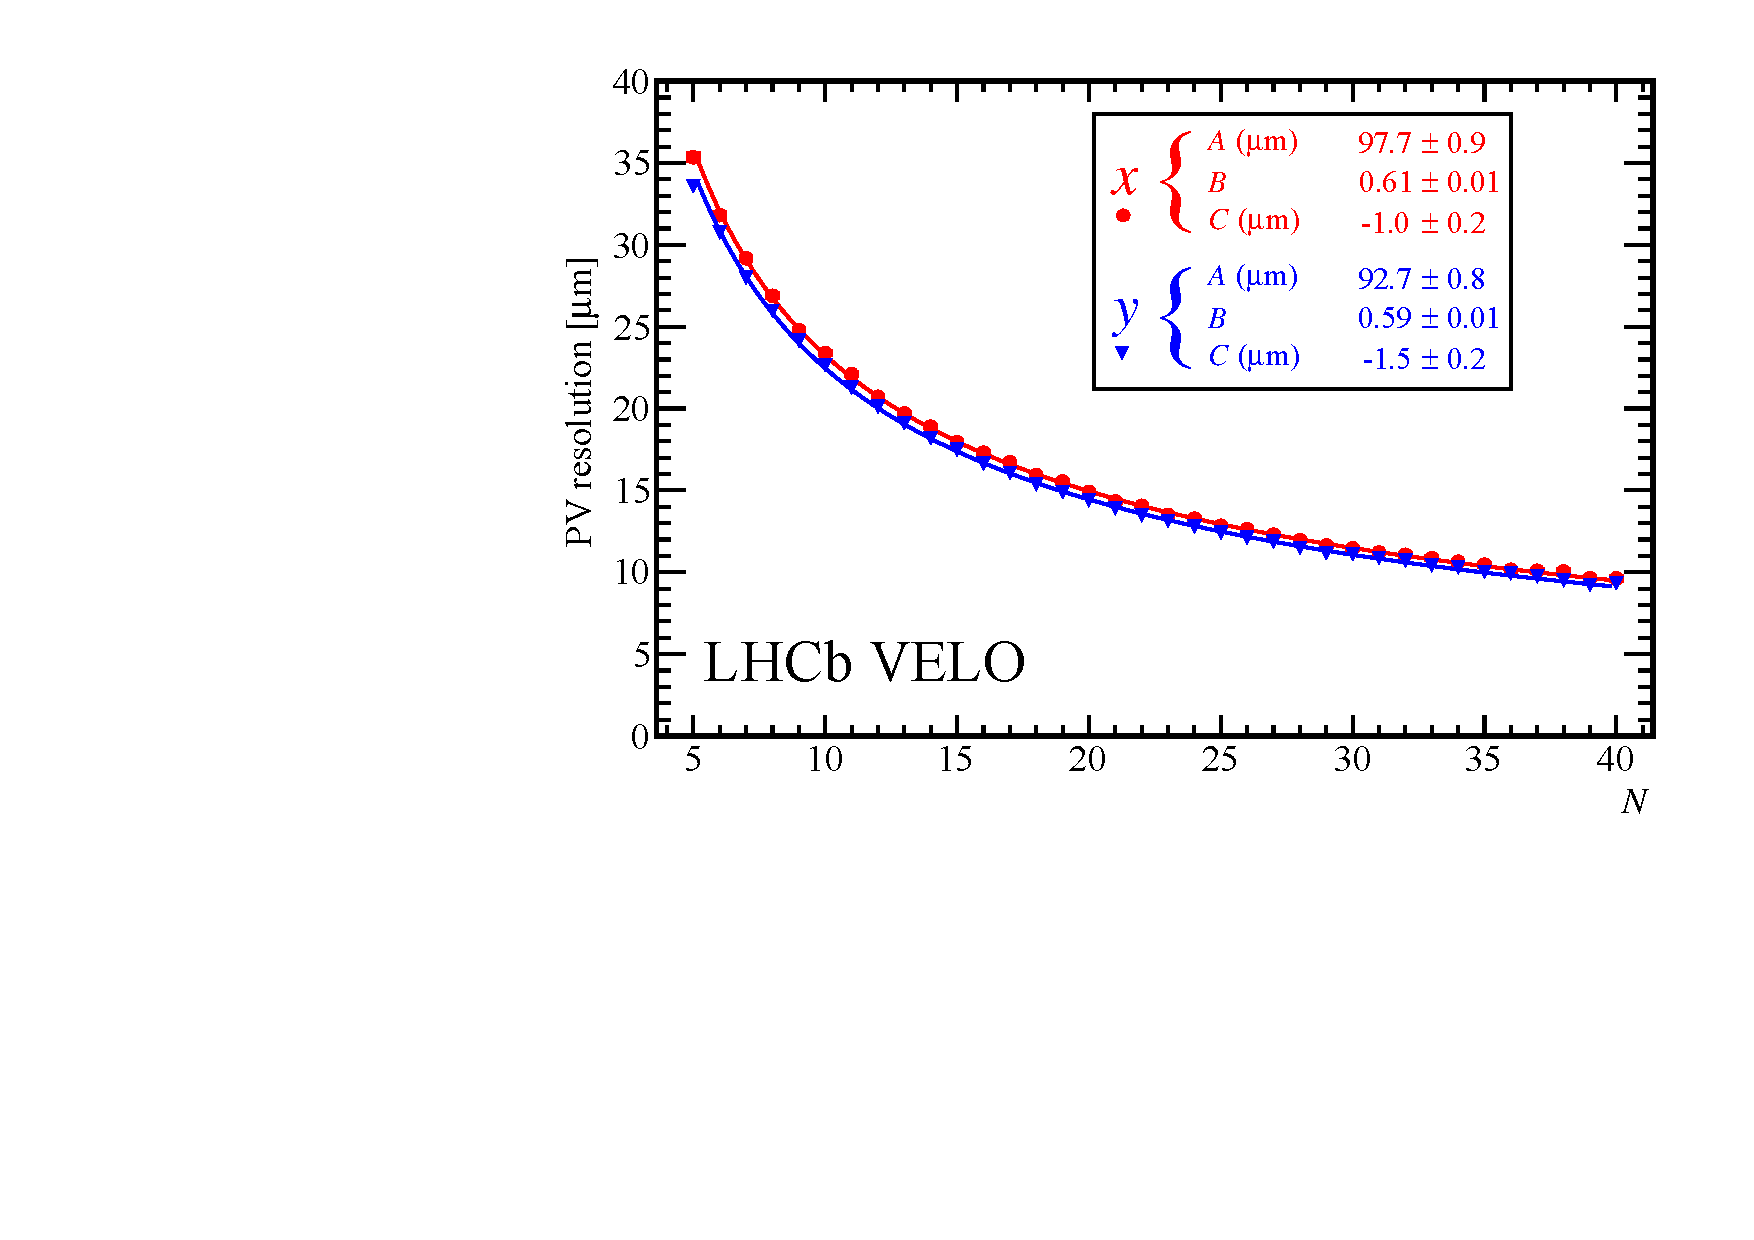
\includegraphics[scale = 0.4]{figs/ResXY_1PV_2011Data}\label{1}}
  \subfloat[]{\includegraphics[scale = 0.4]{figs/ResZ_1PV_2011Data}\label{2}} 
  \caption{The PV resolution in the $x,y$ directions as a function of track multiplicity, $N$, \protect\subref{1}. The PV resolution in $z$ direction as a function of $N$, \protect\subref{2}. The values in the legends refer to the constants in~\autoref{eq:pv} \cite{LHCb-DP-2014-001}.
  }
  \label{fig:PVres}
\end{figure}

\subsection{Reconstructing tracks in the VELO}

The track-finding algorithms in LHCb start in the VELO. Tracks reconstructed in the VELO are then matched with tracks reconstructed from hits in the tracking units further downstream.
The track reconstruction efficiency is defined as the probability that a charged particle passing through the detector (in this case, the VELO) is reconstructed. %This definition of tracking efficiency does not account for interactions with the material, decays in flight and particles that fly outside of the detector acceptance.

The VELO algorithm searches for tracks by looking for clusters in the $R$ sensors consistent with a straight line and then looks for a set of compatible $\Phi$ sensor clusters to reconstruct a trajectory. The minimum number of clusters required to find a track is six (three in the $R$ sensors and three in the $\Phi$ sensors) and the average number of clusters is 11.

The efficiency of the track reconstruction in the VELO is deduced using a tag-and-probe method. Here samples of \jpsi\to\mup\mun decays are used, where one muon is tagged (fully-reconstructed) and the other probe track is partially reconstructed from hits in other parts of the detector. The momenta of the tag and the probe muon are combined to check that it falls within the \jpsi mass window, which is used to confirm the track selection. The VELO efficiency is then obtained by matching the partially reconstructed track to a fully reconstructed track that includes a VELO segment. The absolute efficiency for data for VELO tracks is $\sim$ 98\%. The VELO tracking efficiency observed in the data and in the simulation is shown in~\autoref{fig:velotrack}.


\begin{figure}
  \centering
    \subfloat[]{\includegraphics[scale = 0.35]{figs/Track_Velo_effVsP2011}\label{1}}
      \subfloat[]{\includegraphics[scale = 0.35]{figs/Track_Velo_effVsEta2011.pdf}\label{2}}
    \caption{The tracking efficiency of the VELO for data and simulation as a function of momentum (left) and $\eta$ (right).
  }%note: 2011 data
  \label{fig:velotrack}
\end{figure}

%The discrepancy between data and simulation can be partially explained by certain assumptions made in tracking. Firstly, in the simulation it is assumed that the interaction point is at zero, whereas in data it is offset by 0.4\mm. Secondly the difference in the distance between the two halves of the VELO differ between data and simulation by $\sim$ 150\mum.


\section{The TT station, T station  and track reconstruction}
\label{sec:Tst}
The TT station sits upstream of the dipole magnet and the T stations sit downstream of the magnet. The TT station is roughly 150cm wide and 130cm high and uses silicon micro-strips to detect passing particles. The Inner Tracker (\Gls{IT}) of the T stations is also made of silicon micro-strips and the outer part (the Outer Tracker (\Gls{OT})) of the T stations is made up of straw tubes. The TT, IT and the OT are shown in~\autoref{fig:OT}.
\begin{figure}[h!]
  \centering
  \includegraphics[scale = 0.5]{figs/OuterTracker.png} 
  \caption{The Outer Tracker in the T stations (light blue) made up of straw-modules and the Inner Tracker and TT station (purple) made up of silicon micro-strips \cite{OT}.
  }
  \label{fig:OT}
\end{figure}
Each outer tracker for each T station consists of four layers rotated with respect to the vertical by (0$\degree$, $-$5$\degree$, 5$\degree$, 0$\degree$).

%The rotated layers are referred to as the stereo layers and the non-rotated ones as $x$ layers.

Charged particles must have a momentum of at least 1.5\gevc in order to traverse the magnetic field and reach the T stations. The trajectories of charged particles passing through the detector can be reconstructed from hits in the VELO, T and TT (IT and OT) stations. An example event showing such tracks reconstructed from assigned hits in these stations can be seen in~\autoref{fig:hits}.
\begin{figure}[h!]
  \centering
  \includegraphics[scale = 0.5]{figs/hits} 
  \caption{A display of the reconstructed tracks for an event along with the assigned hits in blue. The insert shows a zoom of the VELO region in the $x$-$y$ plane \cite{det_paper}.
  }
  \label{fig:hits}
\end{figure}

\begin{figure}[h!]
  \centering
  \includegraphics[scale = 0.4]{figs/DOWNUP} 
  \caption{Different types of track in the LHCb detector along with the corresponding magnetic field strength in the $y$ direction \cite{det_paper}
  }
  \label{fig:updown}
\end{figure}
The tracks in LHCb can be characterised into different types, as outlined in~\autoref{fig:updown}. These different track types are:

\begin{description}
\item[Long tracks] which traverse the entire detector. They are defined as tracks which have hits in the VELO and the T stations. Hits in the TT stations are optional. As they traverse the full magnetic field, long tracks offer the most precise momentum measurement and are therefore of most importance to physics analyses. They are also the best understood tracks in terms of efficiency measurements. There are on average 33 long-tracks per event \cite{uksem}. 

\item[Upstream tracks] leave hits only in the VELO and the TT station. This is generally due to the tracks having too low a momentum to reach the T stations. These tracks are not used directly in physics analyses.
%These tracks are only useful for understanding backgrounds in PID algorithms in RICH1 (providing they have a high enough momentum to pass RICH1).

\item [Downstream tracks] like long tracks, are directly used in physics analyses for particles which are long-lived enough to decay outside the VELO, such as $K^{0}_{s}$ and $\Lz$. The reconstruction efficiency of these tracks is poorly understood and part of this thesis focuses on a method to improve this efficiency measurement. There are on average 14 downstream tracks per event.
\item [VELO tracks] pass only through the VELO and are used for PV reconstruction. They are not used directly in physics analyses.
\item[T tracks] pass only through the T stations and tend to be produced in secondary interactions. They are not used directly in physics analyses.  %Again their only use is within the context of RICH2 data treatment for particle identification.
\end{description}

The reconstruction of VELO tracks has already been described. There are two complementary algorithms for adding tracks from downstream detectors to these VELO tracks to make a long track. In the first, so-called forward tracking, the momentum of a particle and its trajectory are entirely determined from a VELO track and a single hit in one of the T stations. Further hits in the T stations which are compatible with this trajectory are then added \cite{forward}. The second algorithm used is referred to as track-matching, where long tracks are made by combining VELO tracks with T tracks, which are found by a stand alone track-finding algorithm \cite{patseed}.

%% Here a track segment is reconstructed in the downstream detectors and then combined with the VELO track. The downstream track segment is formed by requiring that particles leave hits in at least one $x$ and stereo layer in each of the three T stations \cite{match}.

For both algorithms the candidate tracks are combined to form a final set of long tracks. Once combined, hits from the TT station consistent with the trajectory are also added to improve the momentum measurement \cite{tracks}. %The average efficiency to reconstruct long tracks is (97.78 $\pm$ 0.07)\% for 2011 data and (96.99 $\pm$ 0.05)\% for 2012 data \cite{tracks}.

The downstream tracks are reconstructed by taking a stand alone T track and then extrapolating this track through the magnetic field. Once having computed the point at the centre of the magnetic field using the T track, a search for a list of TT measurements making a straight-line with this point is carried out. The main challenges for this method are \gls{ghost} tracks (i.e. hits within the detector which are falsely reconstructed as a track) and the wide window across the TT station within which matching TT measurements must be searched for \cite{downstream}.

%% The efficiency of the downstream track finding algorithm is calculated using simulation. The efficiency for the algorithm to correctly identify a track which has TT and T hits and that is not constructable in the VELO is found to be 46\% Ref.\cite{downstream}. This efficiency increases to 73\% when it is required that the particles reconstructed are daughters of strange mothers produced near the beam line. 

The work described later in this thesis will outline a method to measure the downstream track-finding efficiency using a data-driven method, as a function of $p$ and $\eta$, and will provide a relationship between the downstream tracking efficiency observed in data and the downstream tracking efficiency according to simulation.

%% \section{The \sPlot  technique and $\mathbf{\sWeight}$-ing data}
%% \label{sec:splot}
%% As the following section on the RICH detectors will mention a statistical technique referred to as the \sPlot technique \cite{sPlot}, or \sWeight-ing, the concept is introduced here.

%% The \sPlot technique is used extensively through out this thesis. It is used in cases when one has a merged dataset which consists of data from different sources of data species, namely background and signal. The events in this dataset are assumed to be composed of two different sets of variables. Discriminating variables are those whose distributions are known for background and signal. Control variables are those whose distributions are unknown, or are assumed to be unknown.

%% The \sPlot technique allows the distribution of the control variables for each data species to be deduced by using the species discriminating variable. This method relies on the assumption that there is no correlation between the discriminating variable and the control variable. The discriminating variable used in this thesis is always the mass distribution. The full mathematical description of the \sPlot technique can be seen in Ref. \cite{sPlot}, the key points are outlined here.

%% An unbinned extended maximum likelihood analysis of a data sample of several species is considered. The log-likelihood is expressed as

%% \begin{equation}
%%   \mathcal{L} = \sum^{N}_{e = 1} \left\{\ln \sum^{N_{s}}_{i = 1} N_{i}f_{i}(y_{e})\right\} - \sum^{N_{s}}_{i = 1}N_{i},
%%   \label{eq:ll}
%% \end{equation}

%% where $N$ is the total number of events considered, $N_{s}$ is the number of species of event (i.e. two - background and signal), $N_{i}$ is the average number of expected events for the $i^{th}$ species, $y$ represents the set of discriminating variables and $f_{i}(y_{e})$ is the value of the Probability Density Function (PDF) of $y$ for event $e$ for the $i^{th}$ species. 

%% For the simple (and not particularity practical) case of the control variable $x$ being a function of $y$, i.e. completely correlated, one could naively assume that the probability of a given event of the discriminating variable $y$ being of the species $n$ would be given by

%% \begin{equation}
%%   \mathcal{P}_{n} (y_{e}) = \frac{N_{n}f_{n}(y_{e})}{\sum^{N_{s}}_{k =1} N_{k}f_{k}(y_{e})}.
%% \end{equation}
%% In this scenario the probability would run from 0 to 1.
%% In the case considered in this thesis, where $x$ is entirely uncorrelated with $y$, it can be shown that $\mathcal{P}_{n} (y_{e})$ can be written as

%% \begin{equation}
%%   \mathcal{P}_{n} (y_{e}) = \frac{\sum^{N_{s}}_{j = 1} V_{nj}f_{j}(y_{e})}{\sum^{N_{s}}_{k =1} N_{k}f_{k}(y_{e})},
%%   \label{eq:sw}
%% \end{equation}

%% where $V_{nj}$ is the covariance matrix between the species $n$ and the $j^{th}$ species. The inverse of this covariance matrix is given by the second derivative of -$\mathcal{L}$ in~\autoref{eq:ll}.

%% The quantity in~\autoref{eq:sw} is donated as the \sWeight. In this thesis the species, $n$, in~\autoref{eq:sw} is always the signal. Because of the presence of the covariant derivative the \sWeight of an event can be both positive and negative. The more negative an event is the more likely it is to be background and vice versa for positive \sWeight-s. The signal distribution for the control variable $x$ can then be deduced by histrogramming events in $x$, applying the \sWeight to each event. %Again it is important that the $x$ variable is not correlated with $y$ (that is - the mass distribution).


%% In practice, the \sPlot technique is applied by fitting the background and signal mass distributions in data and using the fitted probability density function (PDF) of the $i_{th}$ species, the total number of events in the data sample, the number of species in the data sample (i.e. two) and the number of average events expected for the $i_{th}$ species, to deduce a weight for each event. These weights range between -1 and 1 .

   
\section{The RICH detectors}
\label{sec:rich}
The main role of the \Gls{RICH} is to provide identification for the charged hadrons $\pi,\kaon$ and \proton. It also provides information on the charged leptons $e$ and $\mu$ which complement the information provided by the calorimeter and muon systems.

%There are two RICH detectors, RICH1 and RICH2, as seen in~\autoref{fig:dec}. Between the two detectors a momentum range of $\sim$1-100\gevc is covered

The momentum of a particle is highly correlated to the polar angle $\theta$, with high momentum particles having a smaller angle. The RICH1 detector system is placed just after the VELO and provides identification for particles with a low momentum range of 2-40\gevc. The RICH2 detector system is placed between the T stations and the first \gls{muonstation}, M1, and covers a momentum range of 15--100\gevc. The RICH2 detector system is placed further downstream, as the higher momentum particles are less affected by the magnet.

The RICH functions on the basis that if a particle travels faster than the speed of light in a medium it will emit Cherenkov radiation. The angle of this radiation is related to the speed of the particle and the refractive index of the medium.  By measuring the Cherenkov angle $\theta_{c}$, the particle mass can be deduced through the relation

\begin{equation}
  \cos\theta_{c} = 1/\beta n  = E/pn =  \frac{\sqrt{m^{2} + p^{2}}}{pn}.
\end{equation}

The radiators used in RICH1 are silica aerogel and $C_{4}F_{10}$. The aerogel has a very low density and high refractive index which makes it ideal for very low momentum particles with momenta $\sim$ \gevc. The aerogel is placed just after the VELO and the rest of the RICH1 is filled with $C_{4}F_{10}$. The optical system in both RICH detectors is similar. A primary spherical tilted focusing mirror and a plane secondary mirror focus and direct the Cherenkov light on to a plane of hybrid photon detectors (HPDs), as shown in~\autoref{fig:rich1}.

%These mirrors focus the Cherenkov radiation of a particle on to the hybrid photon detectors (HPD), as seen in~\autoref{fig:rich1}.

\begin{figure}[h!]
  \centering
  \includegraphics[scale = 0.9]{figs/RICH1diagram.png} 
  \caption{The optical set-up for the RICH1 detector \cite{rich1dia}.
  }
  \label{fig:rich1}
\end{figure}

%There are 2 planes of HPDs in each RICH, with a total of 198 HPDs in RICH1 and 288 in RICH2. 

\subsection{The particle identification algorithm}
A good understanding of the performance of the Particle IDentification (\Gls{PID}) of the RICH is important for the analyses described in this thesis. A precise understanding of the performance  allows the efficiency and mis-identification (mis-id) rate of tracks to be calculated after the RICH information has been applied to the data candidates. To identify effectively the particle type of a track in the RICH, an overall event log-likelihood algorithm is calculated, taking into account all possible hypotheses for all tracks in the event. %s for both rich detectors simulation.

%applied which includes all of the tracks in an event and the information from both RICH detectors simultaneously.

The likelihood minimisation procedure starts by assuming all particles are pions, as pions are the most abundant particle type. The overall event likelihood is calculated from the distribution of the photon hits (which will form rings referred to as Cherenkov rings) along with the event's associated tracks and their errors, assuming the pion mass hypothesis for every track. The mass hypothesis of each track is then changed, one track at a time, whilst leaving the hypothesis for every other track in the event unchanged. The mass hypotheses for $e$, $\mu$, $K$ and proton are applied and the change in mass hypothesis which gives the largest increase in the event likelihood is identified. This method is repeated until no improvement in the event likelihood can be found and thus each track has been set to its preferred hypothesis. Some modifications are made to the logic described above in order to reduce CPU time. The final output of this algorithm is a variable for each track in an event which shows the difference in the total event log-likelihood when the mass hypothesis of the track in question is changed from a pion to $e$, $\mu$, $K$ and proton. These variables are referred to as e.g. \gls{dllkpi}  = $\Delta \text{Log}(\kaon - \pi)$, \gls{dllppi} = $\Delta \text{Log}(\proton - \pi)$ and \gls{dllmupi} = $\Delta \text{Log}(\mu - \pi)$. % and \dllepi = $\Delta \text{Log}(e- \pi)$.
\subsection{The PID performance}
\label{sec:pidperf}
%% The PID performance can be investigated with data, using decays with isolated tracks, whereby the Cherenkov ring from a track does not overlap with other rings. This allows the Cherenkov angle to be uniquely predicted.

The performance of the PID is assessed using data candidates which have been selected without using PID information. Thus decays are needed whereby the individual daughter states can be reconstructed with very little background, using kinematic information alone. The decays chosen include the channels $\PLambda^{0}\to\proton\pim$ and $D^{*+} \to D^{0}(\kaon^{-}\pip)\pip$. These decays have a high purity as can be seen~\autoref{fig:pidcalib}.
\begin{figure}[h!]
  \centering
  %  \subfloat{\includegraphics[scale = 0.23]{figs/kspipi.png}\label{1}}
  \subfloat{\includegraphics[scale = 0.23]{figs/lambdabppi.png}\label{1}}
  \subfloat{\includegraphics[scale = 0.23]{figs/dkpi.png}\label{2}}
  \caption{Fitted invariant mass distributions for $\PLambda^{0}\to\proton\pim$, \protect\subref{1}, and $D^{0}\to \kaon^{-}\pip$, \protect\subref{2} \cite{LHCb-DP-2012-003}.}
  \label{fig:pidcalib}
\end{figure}
The remaining background is removed using the \sPlot technique \cite{sPlot}, which assigns a so-called sWeight (which can be positive or negative) to each event, depending on how signal-like the event is deemed to be.  The \sPlot technique is summarised in~\autoref{sec:splot}.

Using these control samples, the $\text{DLL}_{X\pi}$ distributions are considered for each track type. It is then possible to study the discriminating power of particular PID requirements. The discriminating power of the selection cuts \dllkpi$>0$ and \dllkpi$>5$ placed on tracks with a kaon mass hypotheses can be seen in~\autoref{fig:pid1}\protect\subref{1}. Here the efficiency of these cuts on kaons is shown along with the misidentification of pions as kaons.
 The discriminating power of the selection cuts \dllppi$>0$ and \dllppi$>5$ on tracks with a proton mass hypotheses can be seen in~\autoref{fig:pid1}\protect\subref{2}, along with the mis-id rate of pions to protons and finally the efficiency is shown for $\dllpk>0$, $\dllpk>5$ along with the mis-id rate of kaons to protons in~\autoref{fig:pid1}\protect\subref{3}. In~\autoref{fig:pid1}\protect\subref{3} the variable \dllpk is formed using the relation
\begin{equation}
  \dllpk = \dllppi - \dllkpi.
\end{equation}

\begin{figure}[h!]
  \centering
  \subfloat[]{\includegraphics[scale = 0.8]{figs/kpi_det.png}\label{1}}
      \subfloat[]{\includegraphics[scale = 0.8]{figs/ppi_det.png}\label{2}}\\
      \subfloat[]{\includegraphics[scale = 0.8]{figs/pk_det.png}\label{3}}
      \caption{The kaon efficiency and the misidentification rate for pions as kaons for different PID cuts (filled and hollow markers) \protect\subref{1}, the proton efficiency and the misidentification rate for pions as protons for different PID cuts (filled and hollow markers), \protect\subref{2} and the proton efficiency and the misidentification rate for kaons as protons for different PID cuts (filled and hollow markers), \protect\subref{3} \cite{LHCb-DP-2012-003}.}
  \label{fig:pid1}
\end{figure}

The Cherenkov angle as a function of momentum for tracks passing through the $C_{4}F_{10}$ radiator is shown in~\autoref{fig:cheren}
\begin{figure}[h!]
  \centering
  \includegraphics[scale = 0.9]{figs/cherenkov_angle.png} 
  \caption{Reconstructed Cherenkov angle as a function of track momentum in the $C_{4}F_{10}$ radiator \cite{LHCb-DP-2012-003}.
  }
  \label{fig:cheren}
\end{figure}




%% \begin{figure}[h!]
%%   \centering
%%   \includegraphics[scale = 0.9]{figs/ppi_det.png} 
%%   \caption{The proton efficiency and the misidentification rate for pions as protons for different PID cuts (filled and hollow markers) \cite{LHCb-DP-2012-003}.}
%%   \label{fig:pid2}
%% \end{figure}

%% \begin{figure}[h!]
%%   \centering
%%   \includegraphics[scale = 0.9]{figs/pk_det.png}
%%     \caption{The proton efficiency and the misidentification rate for kaons as protons for different PID cuts (filled and hollow markers) \cite{LHCb-DP-2012-003}.}
%%     \label{fig:pid3}
%% \end{figure}


%% The dependence of the efficiency on momentum and the mis-id rates for varying combinations of pion, proton and kaons can be understood from the variation of $\theta_{c}$ with momentum shown in~\autoref{fig:cheren}. As shown in~\autoref{fig:cheren} the seperation between the kaon and proton hypothesis is less clear for softer protons. Due to this, harder initial cuts are often placed on the proton momentum during off-line analysis. The discriminatory power of a PID cut is also a function of the event multiplicity and $\eta$. 

%% \subsection{The PID calib package}

%% The PID calib package is a collection of files used within the LHCb software which allow the efficiency and mis-identification rates to be calculated for any momentum cut for a particular $\text{DLL}$ variable. These values are calculated using the control channels discussed previously. This package can also be used to reproduce the number of events per PID value for a selected mass hypothesis. These DLL distributions provided by PID calib are binned in terms of momentum, $\eta$ and track multiplicity. The PID calib package provides the $\text{DLL}$ variables \dllppi, \dllkpi \dllmupi and \dllepi. %To deduce the difference in the  log likelihood of a particle with respect to a particle that is not a pion a linear combination of the above $\text{DLL}$ variables can be taken. 

\section{Muon identification}
\label{sec:muonID}
The selection of muons is performed using information from the five muon detector stations M1--5. Each station is divided up into four regions R1--4, all of which cover roughly the same acceptance, as shown in~\autoref{fig:muonst}. The granularity of the station in each region R1--4 reflects the particle density in that region. There is also increased granularity in the $x$ direction, as this is the plane in which particles are bent by the magnetic field.

The M1 station is placed before the \Gls{ECAL} and stations M2--5 are placed downstream of the ECAL. Stations M2--5 are interleaved with 80cm thick iron absorbers. These iron absorbers along with the muon stations M2--5 allow the identification of penetrating muons.
%The final iron filter in~\autoref{fig:muonst} is placed in order to reduced backscattering in the M5 station. 

\begin{figure}[h!]
  \centering
  \includegraphics[scale = 0.9]{figs/MuonStations.png} 
  \caption{The five muon stations (a) (the muon filters refer to iron absorbers - see text) and (b) the station layout in regions R1--4 \cite{muon}.
  }
  \label{fig:muonst}
\end{figure}


%% \subsection{The L0 muon trigger}
%% \label{sec:L0muon}
%% As discussed in~\autoref{sec:L0trig}, the information provided by the muon stations is used in the \Gls{L0} hardware trigger. The L0 muon trigger performs a standalone reconstruction of tracks, requiring hits in all five stations, which allows the $P_{T}$ of a track to be estimated using the hardware alone. The estimation of the track's $P_{T}$ is done by combining tracks in stations M2-5 with hits from M1. The track direction after deflection by the magnetic field can then be determined . The positioning of the M1 further upstream allows a better resolution of the $\pt$ of a given track in the L0 trigger (reducing the resolution from $\sim$35\% to $\sim$25\%) but the M1 station is not used in the high level trigger or off-line reconstruction of tracks.

%Because the muon stations are used in the L0 trigger they are required to send information to the trigger having identified collision events within a time window of 25 $ns$. 

%% Firstly a track is verified in the four stations, M2-5, by searching within suitable areas relative to the interaction point. Then the position of the hits in M2 and M3 are used to predict the position of hits in M1. If a hit is found in M1 within a suitable region the next step is to estimate the \pt of this track to verify whether or not it should pass the trigger.  This done by using the hits in M1 and M2 to find the track direction after deflection by the magnetic. This direction, combined with its impact point at the magnetic centre and the average $pp$ collision point, are used to make a quick estimate of the $\pt$ \cite{muon}. The presence of the M1 further upstream allows a better resolution of the $\pt$ of a given track in the L0 trigger (reducing the resolution from $\sim$35\% to $\sim$25\%) but it is not used in the high level trigger or offline reconstruction of tracks.


\subsection{The efficiency of the muon stations}
As the L0 algorithm requires hits in all five muon stations and an overall efficiency of $>95$\% is desirable, the efficiency of each individual station must be at least 99\%. This is achieved by having a good time resolution and a high detector redundancy. This redundancy is realised by having two independent readouts in many of the stations/regions and requiring a hit in at least one of them and the time resolution to be better than 4ns. All regions of all muon stations fulfil the $>99$\% requirement. %, giving a total muon reconstruction efficiency of $>$95\%. %The efficiency for each muon station as a function of station region is shown in~\autoref{tab:muoneff}.

%% The efficiency of the stations M2-5 are measured by looking at the events which weren't triggered in the HLT or L0 triggers by the muon system. Tracks are then reconstructed using all muon systems minus the one under investigation. These M-tracks are also required to match to good quality high momentum T-tracks. The predicted positions of hits in the M station under investigation, deduced by extrapolation the track already reconstructed from the other stations, are then compared to hits with the M station underinvestgaion in order to deduce the efficiency.

%% For the case of M1 a similar procedure is followed but this time the data comes from \jpsi \to \mup\mun decays, where the muon considered is the one that didn't fire the L0 trigger. This data can be used in the case of M1 because the M1 information is not used in the HLT or offline track reconstructions.


%% \begin{table}
%%   \centering
%%   \hspace*{-0.5cm}
%%   \includegraphics[scale = 0.5]{figs/muonefftab}
%%   \caption{The efficiency to correctly reconstruct a track made by a muon in each region of each muon station. Errors indicate statistical and systematic errors respectively \cite{muon}.}
%%   \label{tab:muoneff}
%% \end{table}

%% The main source of systematic error on the efficiency comes from the modelling of backgrounds whilst calculating the efficiency. 
\subsection{The muon identification procedure}
The  off-line muon identification strategy can be split into three steps \cite{muonID}
\begin{description}
  \item[IsMuon:] A binary selection of muon candidates based on the penetration of the muon candidates through the calorimeters and iron filters is parameterised by the boolean IsMuon variable. There are also momentum requirements, depending on which muon stations have been traversed.  This provides high efficiency, while reducing the misidentification probability of hadrons to the percent level.    
  \item[muDLL:] Based on the pattern of hits around the extrapolation to the different muon stations of the trajectories of charged particles reconstructed in the tracking system, the logarithm of the ratio between the muon and non-muon hypotheses is constructed and used as a discriminating variable, referred to as muDLL. %The pattern of hits around the extrapolated track position allows a computation  of a likelihood for a muon and non-muon hypothesis. The logarithm of the ratio between the muon and non-muon likelihoods gives the discriminating variable muDLL. %in each muon station for IsMuon=true are shown in~\autoref{tab:muonID}. The tracks must also appear in the correct Field of Interest (FOI), i.e. within a certain distance of the extrapolated upstream tracks position in the muon stations.
  \item[$\mathbold{DLL_{\mu\pi}}$:] The RICH information, along with information from the calorimeter, is combined with muDLL to give the discriminating variable \dllmupi.
\end{description}

%% \begin{table}
%%   \centering
%%   \begin{tabular}{l|c}
%%     \hline
%%     Momentum range/(\gevc) & Muon stations\\
%%     \hline
%%     3$<p<$6 & M2 and M3\\
%%     6$<p<$10 & M2 and M3 and (M4 or M5)\\
%%     $p>$10 & M2 and M3 and M4 and M5\\
%%     \hline
%%   \end{tabular}
%%   \caption{Muon stations required to trigger the IsMuon decision as a function of momentum range.}
%%   \label{tab:muonID}
%% \end{table}

\subsection{Efficiency of the muon ID procedure}
The efficiency of the muon selection process is extracted from data, using \jpsi\to\mup\mun decays combined with tag-and-probe techniques. The calculation of the mis-id rates of kaons, pions and protons to muons is performed using the decays outlined in~\autoref{sec:pidperf}. The efficiency for IsMuon, $\epsilon_{IM}$, is shown in~\autoref{fig:isMuon}, along with the mis-id rates as a function of momentum and in ranges of transverse-momentum.

%% the efficiency for finding tracks within the the FOI and which meet the momentum requirements in~\autoref{tab:muonID},

\begin{figure}
  \centering
  \subfloat[]{\includegraphics[scale = 0.3]{figs/Muon1a.png} \label{1}}      
  \subfloat[]{\includegraphics[scale = 0.3]{figs/Muon1b.png}\label{2}}\\
  \subfloat[]{\includegraphics[scale = 0.3]{figs/Muon2a.png}\label{3}}
  \subfloat[]{\includegraphics[scale = 0.3]{figs/Muon2b.png}\label{4}}\\      
  \caption{
 IsMuon efficiency and misidentification probabilities, as a function of momentum and in ranges of transverse-momentum: efficiency of IsMuon on muons, $\epsilon_{IM}$, \protect\subref{1}, IsMuon mis-id rate ($\proton\to\mu$), \protect\subref{2}, IsMuon mis-id rate ($\pion\to\mu$), \protect\subref{3}, and IsMuon mis-id rate ($\kaon\to\mu$), \protect\subref{4} \cite{muonID}.
  }
  \label{fig:isMuon}
\end{figure}

There is a weak efficiency dependence on transverse-momentum. The reason for a more dramatic loss of efficiency for low $P_{T}$ muons is due to the scattering of tracks out of the detector. The mis-id rate also falls with increased transverse-momentum. This is because a higher $P_{T}$ for a given momentum corresponds to a larger polar angle and the track then traverses lower occupancy detector regions \cite{muonID}.

The efficiency of the \dllmupi variable on muons, compared to the mis-id rate for kaons and pions, along with the equivalent distributions for the muDLL variable alone, are shown in~\autoref{fig:dllmupi}.
\begin{figure}[!h]
  \centering
      \subfloat[]{\includegraphics[scale = 0.26]{figs/muontot.png} \label{1}}           \subfloat[]{\includegraphics[scale = 0.26]{figs/muontot1.png}\label{2}}\\
        \caption{Efficiency of selecting muons against the efficiency for selecting pions for the \dllmupi and muDLL variables, \protect\subref{1}. Efficiency of selecting muons against the efficiency for selecting kaons for the \dllmupi and muDLL variables, \protect\subref{2}.
  }
  \label{fig:dllmupi}
\end{figure}
The variables most used in the work presented in this thesis are the IsMuon and $\dllmupi$ variables in combination. 

\section{Simulation}
The analyses described in this thesis rely on an accurate simulation of the physics within the detector, and of the detector itself, in order to correctly model the detector output. The simulation of the detector output can be split into two stages; simulation of the particle decays; and simulation of the detector and the particles interactions with it. In the remainder of this thesis, the simulation of the particles themselves with no detector present is referred to as the generator-level simulation.

The first stage of simulation is to generate $pp$ collisions. These are generated using Pythia 6.4\cite{pythia6} and Pythia 8.1 \cite{pythia8}, which produce sets of outgoing particles produced in the interactions between two incoming particles \cite{pythia6}. The simulated $b\overline{b}$ quark pair is hadronised repeatedly until the relevant $b$-hadron is produced, which for much of  the simulation used in this thesis would be a \Lb baryon \cite{Sam}. Once the relevant $b$-hadron has been simulated, its decay is described by the EvtGen package \cite{Lange:2001uf} which allows for the implementation of form factors and other different physics models. The final state radiation is generated using Photos \cite{photos}. All of these programs, Pythia, EvtGen and Photos are combined to create generator-level simulation. The LHCb detector and the material interactions of particles with the detector are simulated using the Geant4 \cite{Geant4} tool-kit. In the remainder of this thesis, simulation which includes both the detector and the physics simulation is referred to as reconstructed simulation or just simulation.         

%% These $pp$ collisions are generated in almost equal amounts by Pythia 6.4 \cite{pythia6} and Pythia 8.1 \cite{pythia8}.

%% The analysis described in this thesis makes use of simulated data (or pseudodata) events in several areas. Generation of simulated data makes use of existing generic open-source
%% simulation software in a specific LHCb configuration [68].
%% In the first step, pp collision events are generated using Pythia 6.4 [69] and 8.1 [70] in
%% approximately equal measures. The simulated bb quark pair is hadronised repeatedly until
%% a target b hadron4 is produced. The decay of the b hadron is described by EvtGen [71]
%% and final-state radiation is generated using Photos [72]. The particles are then passed
%% through a full simulation of the LHCb detector where the detector model, and the material
%% interactions are implemented using Geant4 [73]. The data from the simulated detector
%% is then stored and reconstructed as if it were real data.
\clearpage
